\section{Methods}
\begin{frame}{Particle Filter Setup}
\begin{itemize}
    \item Weighting function
        \begin{itemize}
            \item Continuous, Long Tailed, Zero-Mean 
            \item Too wide $\rightarrow$ under-sensitivity, 
                slow or no convergence
            \item Too thin $\rightarrow$ reduces robustness 
                to noise, particle deprivation
            \item For this work, $N(0, 0.005^2)$ used
        \end{itemize}
    \item Resampling 
        \begin{itemize}
            \item Stratified Resampling can result in truncated tails 
                    on posterior
            \item Regularized Resampling can result in over smoothing and 
                    slow convergence
            \item Resampling Performed Rarely
        \end{itemize}
    \item Number of particles
        \begin{itemize}
            \item More particles give higher fidelity 
            \item Large Initial Particle Count (16000)
        \end{itemize}
    \item Prior Distribution
    \begin{itemize}
            \item Large $\tau$ parameters can oversmooth
            \item $\epsilon$ needs large variance
    \end{itemize}
\end{itemize}
\note{Because the first 20 measurements drop most weights very quickly this gives a large breadth,
    but after the initial calculations drops the computation requirements}
\note{This has not been done before}
\end{frame}

\begin{frame}{FMRI Noise}
\centering

Resting State Noise

\includegraphics[trim=3cm 0cm 3cm 0cm,width=.75\textwidth]{noise2_0009_22_38_23}

Resting State Noise Steps

\includegraphics[trim=3cm 0cm 3cm 0cm,width=.75\textwidth]{noise2_0009d_22_38_23}

\note{Tanabe 2002 \autoref{Tanabe2002} 10-15\% of voxels exhibit significant drift}
\note{Occurs in Cadavers.}
\end{frame}

\begin{frame}{Preprocessing}
  \begin{columns}
    \begin{column}{.6\textwidth}
        \begin{itemize}
            \item Drop Initial Volumes (9, $18.9$s)
            \item Realign Over Time
            \item Detrend (SPM uses $1/128 Hz$ cut off)
            \item Gaussian Smoothing (SPM Only)
            \begin{itemize}
                \item Imposes Gaussianity
                \item Increases SNR
                \item Reduces Bonferroni Correction Requirement
            \end{itemize}
        \end{itemize}
    \end{column}
    
    \begin{column}{.4\textwidth}
        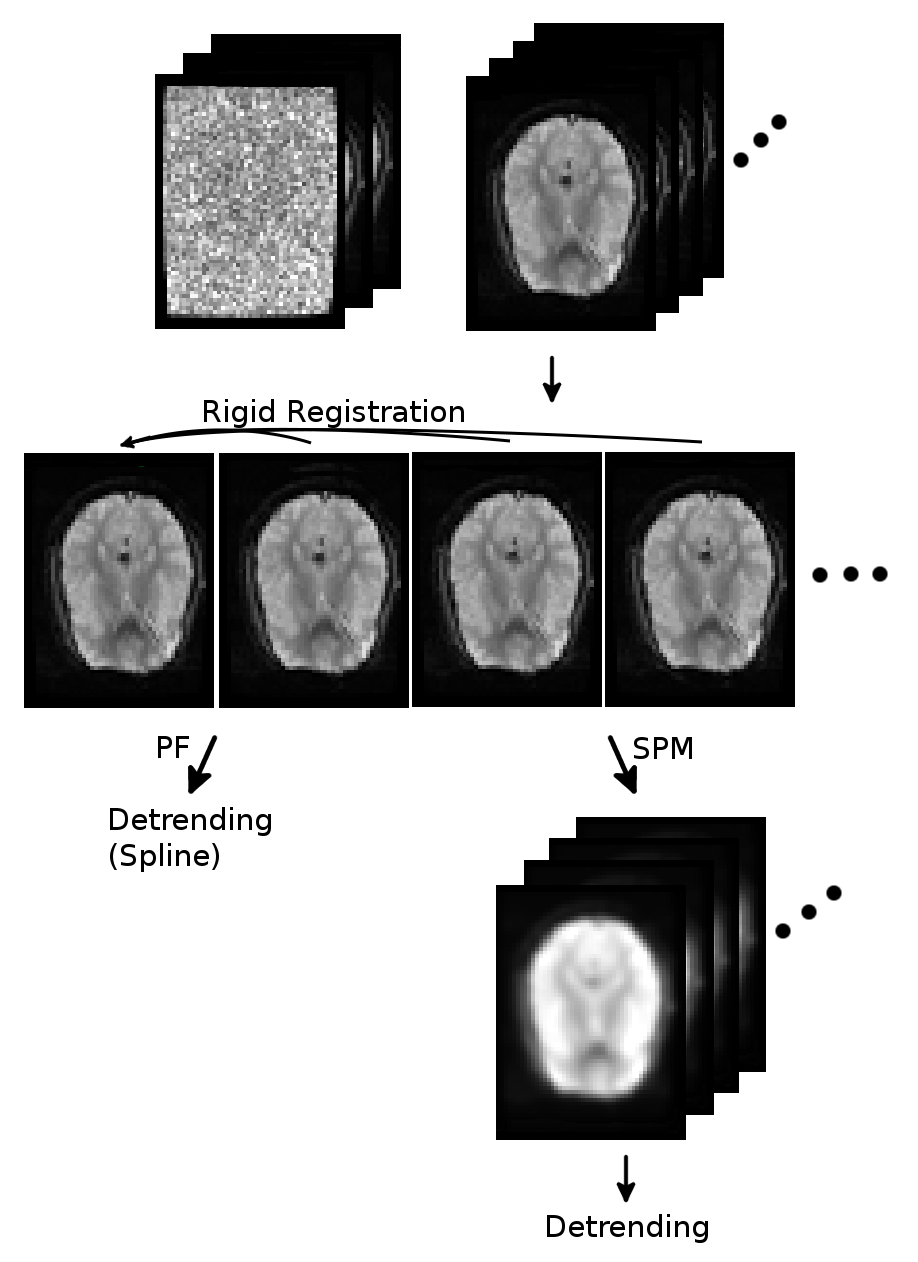
\includegraphics[width=\textwidth]{preprocess}
    \end{column}
  \end{columns}
\end{frame}

